% ------------------------------------------------------------------------
% ------------------------------------------------------------------------
% ------------------------------------------------------------------------
%                                Capítulo 2
% ------------------------------------------------------------------------
% ------------------------------------------------------------------------
% ------------------------------------------------------------------------

\chapter{FUNDAMENTO TEÓRICO/CONCEPTOS FUNDAMENTALES}
% ------------------------------------------------------------------------
\section{Perovskita tipo Ruddlesden-Popper}

La familia de estructuras tipo Ruddlesden-Popper (\textsc{rp}) consiste en capas de bloques de perovskita dislocadas sobre el plano. Dentro de la familia \textsc{rp} con fórmula química $A_{n+1}B_{n}X_{3n+1}$, existen fases diferenciadas por el valor $n$, que estructuralmente indica cada cuantas capas se presentan las dislocaciones \cite{Tobias2004}. En la figura \ref{Fig. series-rp}a se muestran 3 fases de la familia \textsc{rp}, para $n=1$, las dislocaciones se dan capa, mientras que para la fase $n=2$ y $n=3$ las dislocaciones se dan cada dos y tres capas, respectivamente \cite{Fuertes2012ChemistryPerovskites}.
A diferencia de la perovskita cúbica $ABX_{3}$, la fase (\textsc{rp}) $n=1$ tiene fórmula química $A_{2}BX_{4}$ ó $(AX)(ABX_{3})$, donde $A$ y $B$ representan los cationes, y $X$ son los aniones de la estructura \cite{Beznosikov2000}. La fase \textsc{rp} es considerada como capas de bloques de perovskita $ABX_{3}$ dislocadas en la dirección [110] debido a la existencia de mas contenido $AX$ \cite{Suemoto2018IntergrowthSr2TaO3N}. Es decir, los octaedros de la perovskita se arman por capas pero con desviaciones locales. Algunos ejemplos de los sistemas por capas son: $(Sr,Ca)_{3}Sn_{2}O_{7}$ \cite{Yoshida2018HybridPhases}, $Ca_{3}Nb_{2}N_{2}O_{5}$ \cite{Gou2020Photocatalysis}, $K_{2}MgF_{4}$, $Nd_{2}CuO_{4}$ \cite{Beznosikov2000}.

La figura \ref{Fig. series-rp}(b-c) muestra la disposición de los átomos en la celda unitaria. Los elementos que ocupan los sitios cristalográficos son: los cationes estroncio $(Sr)$ para el sitio $A$, niobio ó tántalo $(Nb/Ta)$ para el sitio $B$, y oxigeno $(O)$ para el sitio $X$. Las dos estructuras cristalinas de la fase \textsc{rp} de alta simetría son $Sr_{2}TaO_{4}$ y $Sr_{2}NbO_{4}$, identificadas con el grupo de simetría espacial 139 llamado $I4/mmm$, perteneciente al tipo de estructura tetragonal \cite{Clarke2002}.

\begin{figure}[H]
    \centering
    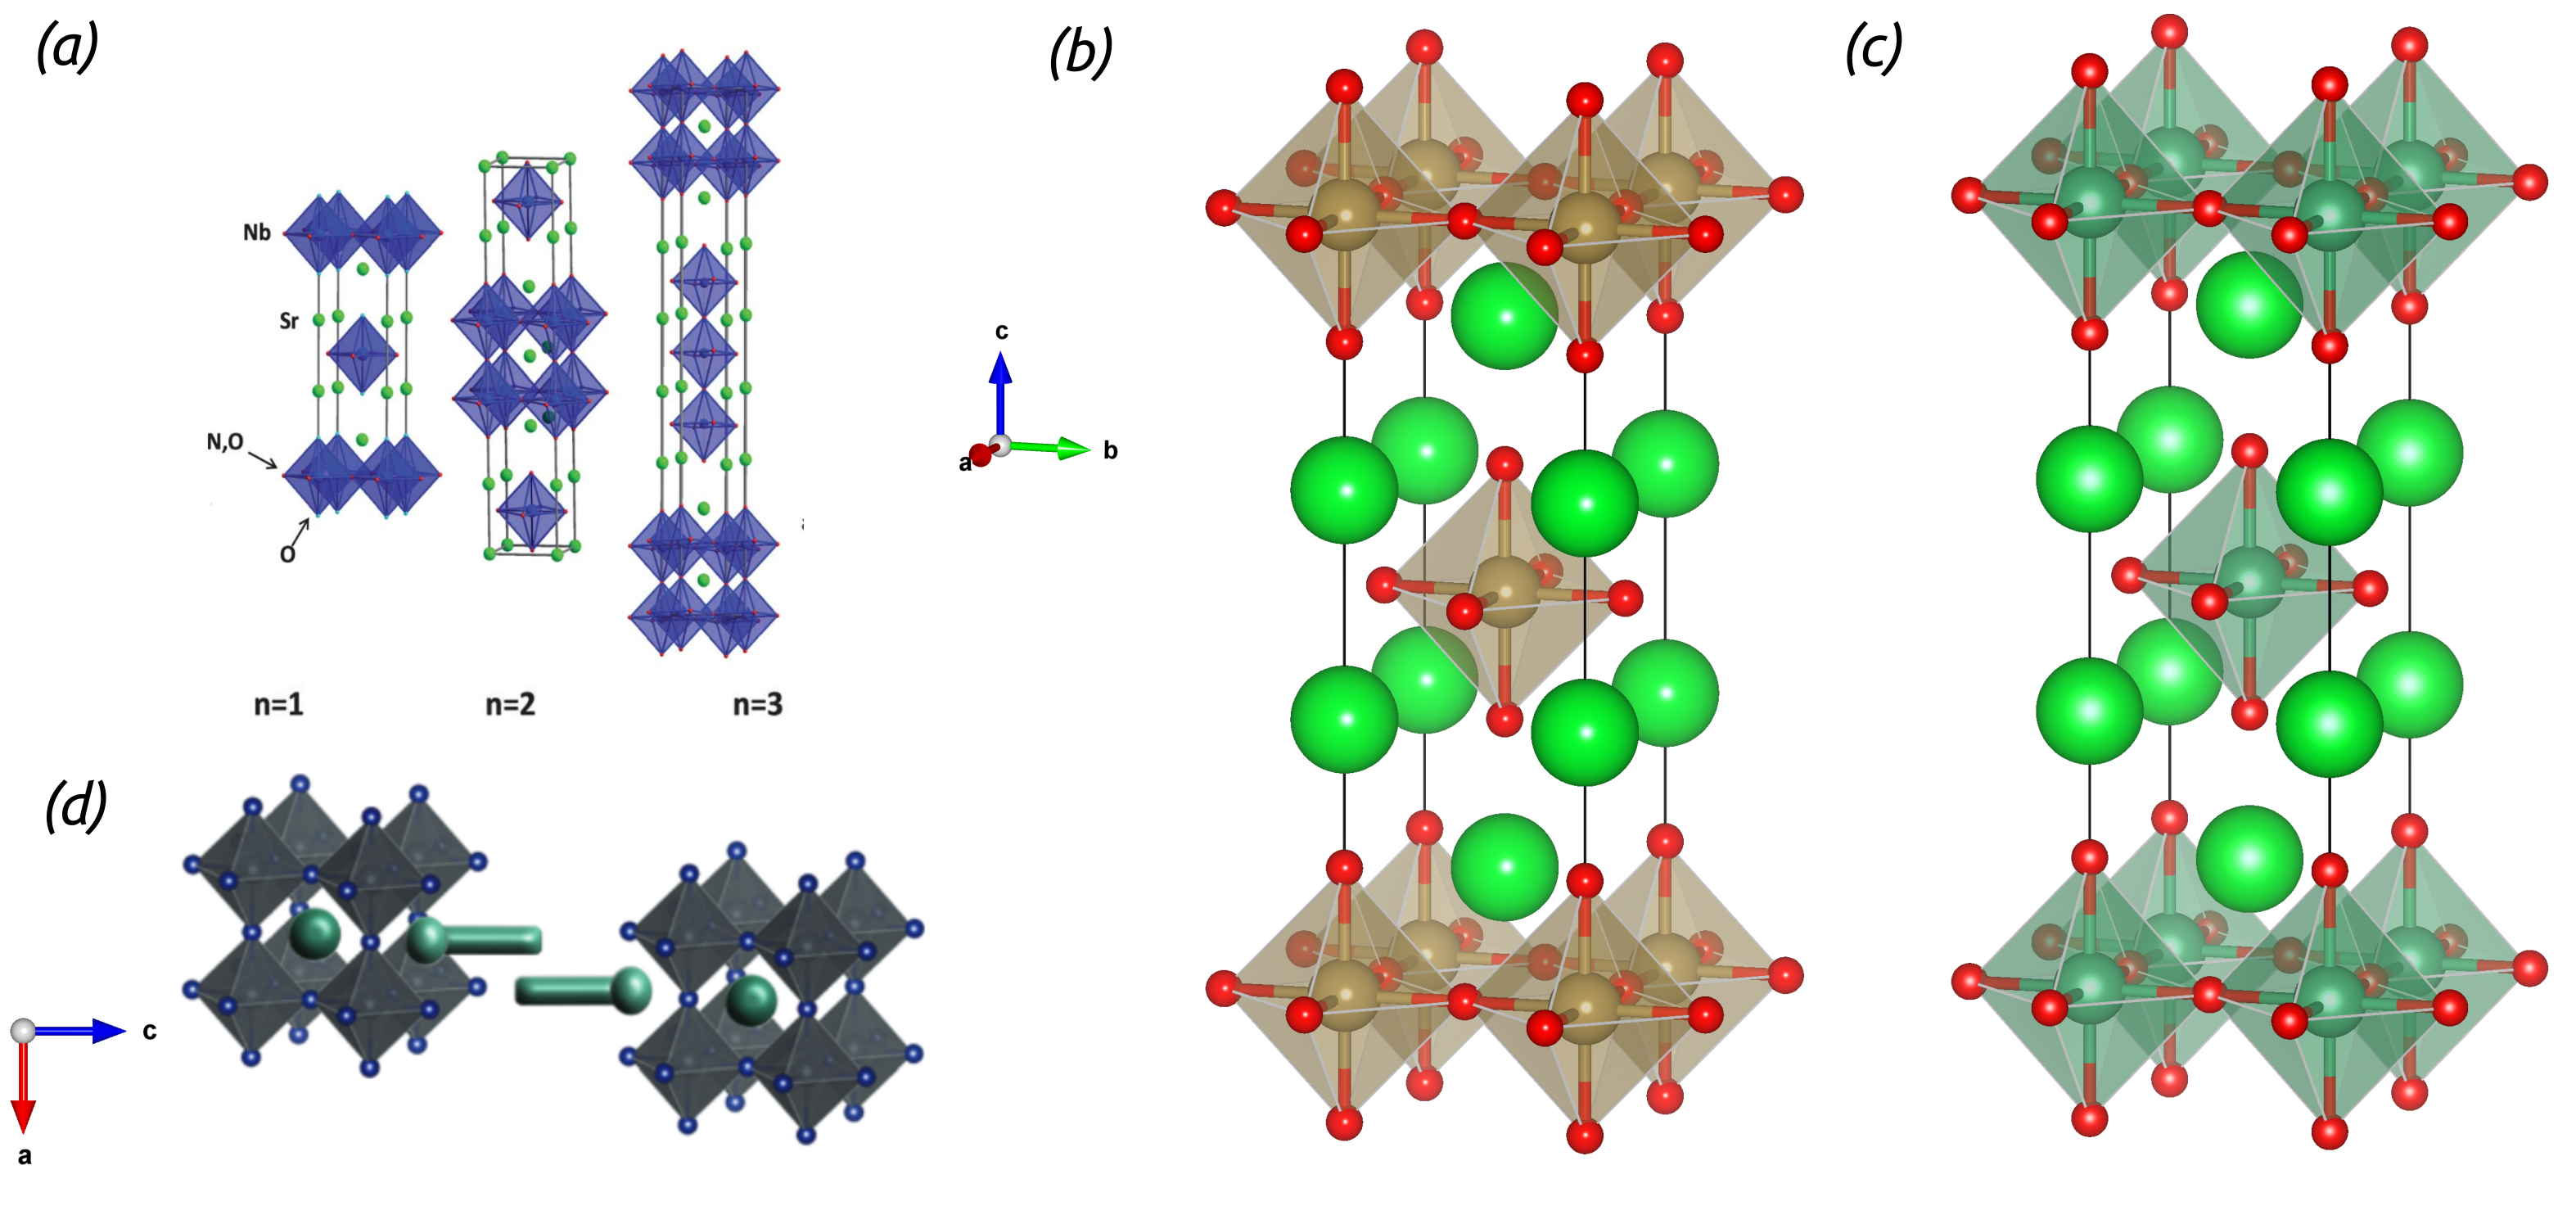
\includegraphics[width=13.0cm,keepaspectratio=true]{Figs/series-rp.png}
    \caption{Celda unitaria de la familia Ruddlesden-Popper para: (a) tres fases $(SrO) (SrNbO_{3})$ \cite{Fuertes2012ChemistryPerovskites}, la fase $n=1$ de (b) $Sr_{2}TaO_{4}$ y (c) $Sr_{2}NbO_{4}$. (d) Esquema estructural de \textsc{rp} \cite{milic2021Multi}.}
    \label{Fig. series-rp}
\end{figure}

En general, la investigación en sistemas por capas se ha extendido debido a posibles propiedades contenidas en los espacios entre capas dislocadas. Un ejemplo de ello es la tendencia por buscar nuevas fases superconductoras de sistemas laminares con metales de transición distintos del cobre\cite{Maeno1994SuperconductivityCopper}. En el caso de la familia Ruddlesden-Popper, el rompimiento del enlace debido a la dislocación de las capas (ver figura \ref{Fig. series-rp}d) permite aprovechar el espacio generado para enlazar elementos o moléculas, como lo evidencia Milić y su trabajo con materiales de perovskita de haluro por capas conectadas por restos orgánicos \cite{milic2021Multi}.  

\section{Oxinitruros}

Los oxinitruros tipo perovskitas son una clase emergente de material con propiedades ópticas, eléctricas, foto-catalíticas\cite{Pan2015Innentitelbild:10/2015}, dieléctricas y magnetorresistivas que pueden ser sensibles al orden óxido-nitruro. Se caracterizan por la disposición de los aniones de oxígeno y nitrógeno en las esquinas de los octaedros de la perovskita, lo que genera diferentes ordenamientos de oxígeno-nitrógeno en el octaedro, nombrados \emph{fac}, \emph{mer}, \emph{trans} y \emph{cis} (figura \ref{Fig. cis_fac_mec_trans}). El oxigeno y el nitrógeno tienen similitudes en electronegatividad, polarizabilidad, radio iónico y numero de coordinación, permitiendo la formación de fases similares cuando son combinados en una misma estructura\cite{Tobias2004,Yang2011}.

\begin{figure}[H]
    \centering
    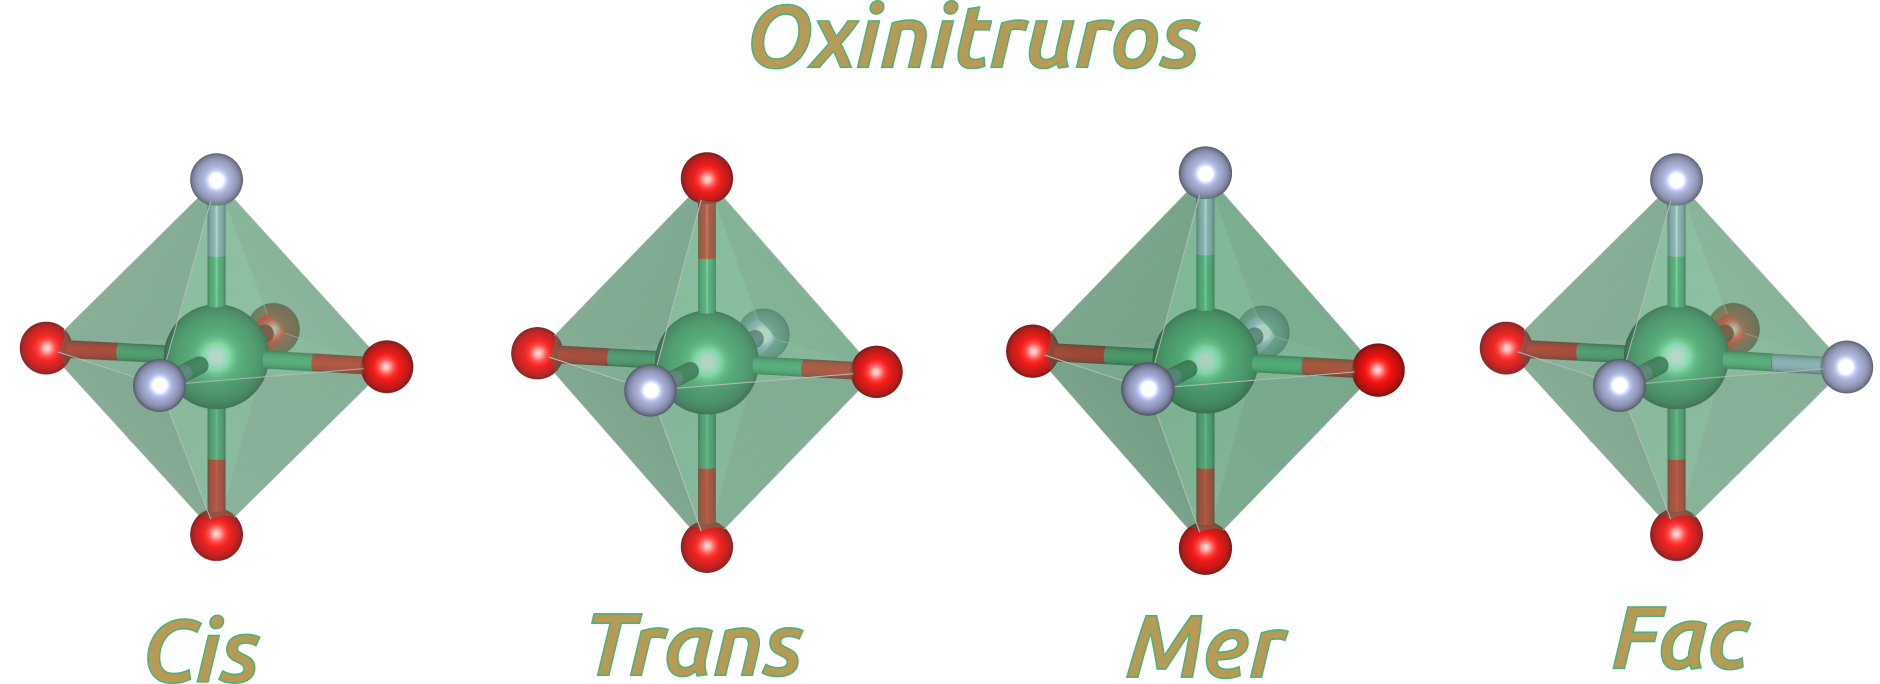
\includegraphics[width=8.0cm,keepaspectratio=true]{Figs/cis_trans_mer_fac.png}
    \caption{Combinación del oxígeno y el nitrógeno en el octaedro de la perovskita. Por notación, los aniones de oxigeno y nitrógeno son denotados en colores rojo y gris respectivamente.}
    \label{Fig. cis_fac_mec_trans}
\end{figure}

Su estabilidad a temperatura ambiente es mayor comparada con los nitruros puros, pero con brechas en la banda electrónica más pequeñas comparadas con los óxidos. Esto conduce al mejoramiento de propiedades ópticas y electrónicas que puedan existir en el material, tales como el dopado de nitrógeno ($N$) en el material $TiO_{2}$. El enlace covalente de $\text{metal}-N$ junto con el enlace $\text{metal}-O$ conlleva a una reducción de la brechas en la banda electrónica, permitiendo el ajuste de la absorción de luz desde la región ultravioleta a la región visible\cite{Gou2020Photocatalysis} para la fotocatálisis\cite{Ebbinghaus2004,Yang2011}.

La búsqueda de fotocatalizadores de luz visible para la división general del agua en hidrógeno y oxígeno es una tarea desafiante para resolver la crisis energética y la contaminación ambiental \cite{Cen2019OptimizedSplitting}. Por lo tanto, es muy deseable explorar oxinitruros de perovskita ferroeléctricos para fotocatálisis de alto rendimiento. A pesar de que estos sistema son la tecnología más nueva y han atraído nuevas investigaciones importantes sobre la generación de hidrógeno, hasta ahora, no se han realizado muchas investigaciones sobre materiales ferroeléctricos para su uso en sistemas de división de agua \cite{Gou2020Photocatalysis}, diseñando nuevas fases que se basan en sustituir el oxigeno por un anión similar en polarizabilidad y electronegatividad como el nitrógeno\cite{Rossell2012Auth}. La gran mayoría de oxifluoruros y oxinitruros exhiben ordenamientos aniónicos \emph{cis} y \emph{fac}, aunque estudios recientes han demostrado que puede inducir el orden de aniones \emph{trans}\cite{Harada2019}.



%\section{Motivación}

%A continuación se presentan dos interesantes propiedades del material perovskita tipo Ruddlesden-Popper: ferroelectricidad y actividad catalítica mediante luz para división de agua.

\section{Ferroelectricidad}

El concepto básico de ferroelectricidad fue introducido por Valasek en el sistema \textit{sal de Rochelle} en 1920 \cite{Valasek1921Piezo-electricSalt}: si se aplica un campo eléctrico externo a un material ferroeléctrico, los dipolos en la estructura cristalina son inducidos a producir una polarización espontánea y alineación con el campo externo, incluso cuando el campo eléctrico está apagado el material tiene polarización remanente que es su polarización espontánea. A esto se le llama fenómeno ferroeléctrico \cite{Kim2018FerroelectricSplitting}. En términos generales, el mecanismo de los ferroeléctricos puede ser categorizado en dos tipos: (1) de orden-desorden, para el cual la reorientación de iones de un estado desordenado a un estado ordenado conduce a la ferroelectricidad  y (2) de desplazamiento, para lo cual la ferroelectricidad surge del desplazamiento relativo de iones \cite{Kim2018FerroelectricSplitting,Shi2016SymmetryFerroelectrics}. 

En los sistemas cristalinos, hay $31$ grupos de punto que describen las simetrías de las estructuras cristalinas. estos grupos contienen transformaciones u operaciones de simetría como traslación, inversión, reflexión y rotación \cite{Glazer2013SpaceScientists}. De los $31$ grupos de punto solo $10$ son grupos polares, formalmente definidos como grupos con estructura no centro-simétrica. Esta definición es indispensable para hablar de sistemas ferroeléctricos, la estructura cristalina puede obtener una pequeña distorsión que rompe la simetría implicando un desplazamiento polar en los átomos de la celda unitaria. Los materiales ferroeléctricos son inseparables del rompimiento de simetría exhibiendo un fenómeno de transición de fase. Este rompimiento de la simetría es capturada por el parámetro de orden conocido como polarización espontánea que puede ser presentada en una fase con grupo de punto polar \cite{Rabe2007ModernFerro}. La transición de fase se lleva desde una fase paraeléctrica de alta temperatura y alta simetría a una fase ferroeléctrica de baja temperatura y baja simetría. En la fase paraeléctrica, existe una relación lineal entre la polarización (P) y el campo eléctrico (E), mientras que la curva no lineal que emerge en la fase ferroeléctrica se conoce como  curva de histéresis ferroeléctrica \cite{Shi2016SymmetryFerroelectrics} (figura \ref{Fig. p-e}). 

\begin{figure}[H]
    \centering
    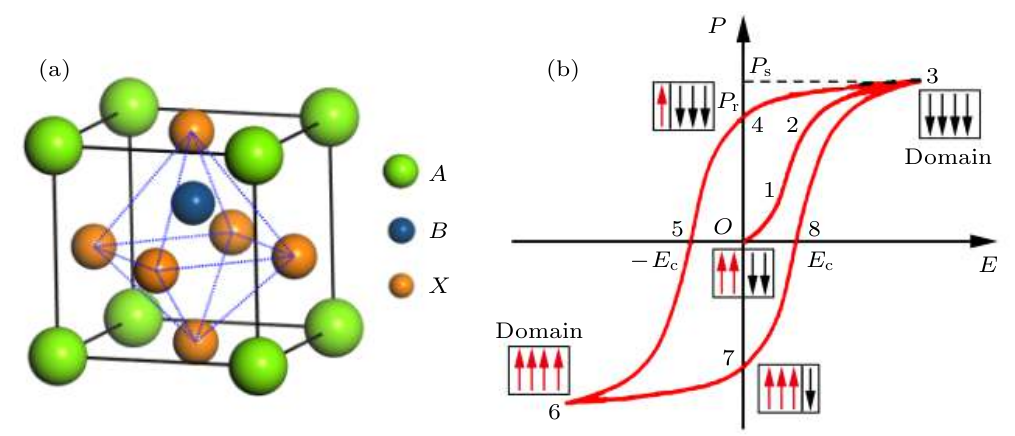
\includegraphics[width=0.9\textwidth]{Figs/polarization.png}
    \caption{(a)Estructura $ABX_{3}$ tipo perovskita. (b) Curva de histéresis \textsc{p-e} \cite{Cui2020ResearchSemiconductors}.}
    \label{Fig. p-e}
\end{figure}

Los materiales ferroeléctricos tienen propiedades útiles con un amplio rango de aplicabilidad. Algunos ejemplos son: Películas delgadas de $SrBi_{2}Ta_{2}O_{9}$ aplicada a memorias de acceso aleatorio ferroeléctricas (\textsc{fram}) \cite{Sreenivas1994film}. El material $LiNbO_{3}$ ferroeléctrico que exhibe fuertes efectos electro-ópticos aplicables en fotónica \cite{Whatmore2021celebrration}. Los oxinitruros de perovskita son aplicables como materiales ferroeléctricos \cite{Bouri2018} debido a la disposición e interacción entre el orden de aniones promoviendo ferroelectricidad \cite{Gou2020Photocatalysis,Yang_2015}, experimentalmente confirmado en la superficie de los materiales $SrTaO_{2}N$ y $Sr_{2}TaO_{3}N$\cite{Suemoto2018IntergrowthSr2TaO3N}. 

\section{Fotocatálisis}

La conversión directa de la luz solar en combustibles químicos mediante reacciones electroquímicas representa una alternativa limpia, sostenible y potencialmente barata a los combustibles fósiles, además de ser una tarea muy desafiante para resolver la crisis energética y la contaminación ambiental \cite{Cen2019OptimizedSplitting}. La reacción más simple de este tipo es la reacción de división de agua en la que el agua se divide en hidrógeno y oxígeno \cite{Castelli_2013}. Durante la fotocatálisis, el fotón absorbido excita un electrón a la banda de conducción, dejando un hueco en la banda de valencia. Los electrones y huecos foto-generados migrarán a la superficie para contribuir a la reducción y oxidación de las especies absorbidas, lo que finalmente resulta en la producción de $H_{2}$ y $O_{2}$ \cite{Bouri2018}.

Cualquier material empleado como fotocatalizador para división de agua debe cumplir con un conjunto de criterios: estabilidad química y estructural, una banda prohibida en el rango visible con un intervalo de banda óptimo ($\sim2eV$) \cite{Cen2019OptimizedSplitting}, bordes de banda bien posicionados con respecto a los niveles red-ox del agua, y alta movilidad de electrones y huecos. Además, se requieren bajos costos y no toxicidad \cite{Castelli_2013}. Los oxinitruros son prometedores fotocatalizadores \cite{Suemoto2018IntergrowthSr2TaO3N,kato2001,wang2015} debido a que contienen aniones con electronegatividad más débil en relación con el oxigeno ($O$), exhibiendo brechas de banda electrónica más pequeños que los óxidos de perovskita, lo que ajusta la absorción óptica desde el ultravioleta al rango visible del espectro solar \cite{Fuertes2015}. Entre los oxinitruros, la brecha de la banda electrónica reducida debido a la sensibilidad del orden oxinitrado \cite{Tobias2004,Yang2011} y la ferroelectricidad benefician la separación de pares de electrones-huecos foto-excitados, permitiendo que estructuras \textsc{rp} como $A_{2}BO_{3}N$ ($A=Cs,Ca,Sr,Ba$ y $ B=Ta,Nb)$ \cite{Cen2019OptimizedSplitting,Pan2018} muestren un rendimiento fotocatalítico prometedor en el espectro visible \cite{Gou2020Photocatalysis,siritanaratkul2011,ZHANG2019}.


\section{Teoría Funcional de la Densidad (DFT)}

La teoría funcional de la densidad es la base para los cálculos de optimización de la estructura, cálculos auto-consistentes de la estructura electrónica y estructura fonónica. Además, se tendrá en cuenta un término adicional llamado parámetro de Hubbard (\textsc{u}) para sistemas altamente correlacionados, debido a la correlación de los electrones en los metales de transición niobio ($Nb$) y tántalo ($Ta$) \cite{Tolba2018}.

La idea fundamental de la teoría funcional de la densidad consiste en que cualquier propiedad de un sistema de muchas partículas interactuantes puede ser visto como una funcional de la densidad del estado base $n_{0}(\Vec{r})$, es una teoría de un sistema de muchos cuerpos correlacionados y ha llegado a ser la herramienta principal para cálculos de estructura electrónica y otros sistemas finitos \cite{martin_2004}. La idea original parte del método de Thomas-Fermi\cite{Fermi1927StatisticalAtoms,Thomas1927TheFields}, la energía cinética de un sistema de electrones es aproximada como una funcional explicita de la densidad, idealizada como electrones no interactuantes en un gas homogéneo con densidad igual a la densidad local en cualquier punto dado. Tanto Thomas como Fermi no tuvieron en cuenta el intercambio y la correlación entre electrones, sin embargo, esto fue agregado por Dirac\cite{Dirac1930NoteAtom} en 1930, quien formuló la aproximación local para el intercambio de electrones.

\begin{equation}
    E_{TF}[n]=\int n(\vec{r})^{5/3}\mathrm{d}^{3}r+\int V_{ext}(\vec{r})n(\vec{r})\mathrm{d}^{3}r+ \int n(\vec{r})^{4/3}\mathrm{d}^{3}r+\frac{1}{2}\int  \frac{n(\vec{r})n(\vec{r'})}{|\vec{r}-\vec{r'}|}\mathrm{d}^{3}r
\end{equation}

El primer término es la aproximación local de la energía cinética, el tercer termino es el intercambio local y el ultimo termino es la energía electrostática de Hartree. La densidad y energía del estado base puede ser encontrado minimizando la funcional $E[n]$ para todos los posibles $n(\vec{r})$ sujeto a la restricción sobre el numero total de electrones.

\begin{equation}
    N=\int n(\vec{r})\mathrm{d}^{3}r
\end{equation}

Esta es una primera aproximación de la teoría funcional de la densidad, pero Hohenberg y Kohn le dan el enfoque para formular esta teoría como un teoría exacta de sistemas de muchos cuerpos. La formulación aplica para cualquier sistema de partículas interactuantes en un potencial externo $V_{ext}(\vec{r})$, incluyendo cualquier problema de electrones y núcleos fijos, donde el hamiltoniano puede ser escrito como:

\begin{equation}
    \hat{H}=-\frac{\hslash^{2}}{2m_{e}}\sum_{i}\nabla_{i}^{2}+\sum_{i}V_{ext}(\vec{r}_{i})+\frac{1}{2}\sum_{i\neq j}\frac{e^{2}}{|\vec{r}_{i}-\vec{r}_{j}|}
    \label{Eq. Hamiltonian_HK}
\end{equation}

\subsection{Teoremas de Hohenberg-Kohn}

La teoría funcional de la densidad esta basada en dos teoremas primeramente demostrados por Hohenberg y Kohn\cite{P.Hohemberg1964InhomogeneousGas}:

\begin{itemize}
    \item \textbf{Teorema 1:} Para cualquier sistema de partículas interactuantes en un potencial externo $V_{\text{ext}}(\vec{r})$, este potencial es determinado únicamente por la densidad de partículas del estado base $n_{0}(\vec{r})$.
    \item \textbf{Teorema 2:}  Una funcional universal para la energía $E[n]$ en términos de la densidad $n(\vec{r})$ puede ser definida, valida para cualquier potencial externo $V_{\text{ext}}(\vec{r})$. Para cualquier potencial particular $V_{\text{ext}}(\vec{r})$, el valor de energía exacta del estado base del sistema es un mínimo global de esta funcional, y  la densidad $n(\vec{r})$ que minimiza el funcional es la densidad exacta del estado base $n_{0}(\vec{r})$.
\end{itemize}

%\begin{itemize}
%   \item \textbf{Corolario 1:} Todas las propiedades del sistema están completamente determinadas dando solo la densidad del estado base $n_{0}(\vec{r})$.
%    \item \textbf{Corolario 2:} El funcional $E[n]$ es suficiente para determinar la energía y la densidad exacta del estado base.
%\end{itemize}

En principio, las funciones de onda $\Psi$ de cualquier estado están determinadas resolviendo la ecuación de Schrodinger con el hamiltoniano presente en la ecuación (\ref{Eq. Hamiltonian_HK}).  Entre todas las soluciones las cuales son consistentes con la densidad dada, la única función de onda $\Psi$ del estado base es la que tiene la menor energía. El teorema solo requiere que la densidad electrónica determine de forma única la posición y los tipos de núcleos, lo cual puede ser probado fácilmente desde la mecánica cuántica elemental. Pero aún existe el problema original de muchos electrones interactuantes moviéndose en el potencial debido a los núcleos. Como todas las propiedades del sistema, son determinadas de forma única si $n(\vec{r})$ es especificado, entonces cada propiedad puede ser vista como una funcional de $n(\vec{r})$, incluyendo la funcional de la energía total:

\begin{equation}
    \begin{split}
        E_{\textsc{hk}}[n]&=T[n]+E_{\text{int}}[n]+\int\mathrm{d}^{3}rV_{\text{ext}}(\vec{r})n(\vec{r})+E_{\textsc{ii}}\\
        &=F_{\textsc{hk}}[n]+\int\mathrm{d}^{3}rV_{\text{ext}}(\vec{r})n(\vec{r})+E_{\textsc{ii}}
    \end{split}
    \label{Eq. E_HK}
\end{equation}

Donde $E_{\textsc{ii}}$ es la energía de interacción del núcleo, el termino $F_{\textsc{hk}}[n]$ incluye  las energías internas, cinética y potencial del sistema de electrones. Entonces un funcional puede ser definido por cualquier densidad, y minimizando este funcional se puede encontrar la densidad y la energía exacta para un sistema interactuante de muchos cuerpos \cite{martin_2004}. Un interesante punto es que un sistema con una polarización neta con campo eléctrico $\vec{E}=0$ como lo es un ferroeléctrico, la polarización es determinada solo por la densidad\cite{Martin1997FunctionalSystems,Martin1997RecentSolids}, es decir el teorema original de Hohenberg-Kohn si aplica. Los teoremas están en términos de funcionales de la densidad desconocidos, y es demostrable que estos deben ser funcionales no locales, dependiendo simultáneamente sobre $n(\vec{r})$ con posiciones diferentes de $\vec{r}$. Si el funcional $F_{\textsc{hk}}[n]$ es conocido, se puede minimizar la energía total del sistema respecto a las variaciones en la densidad electrónica, y se podría encontrar la densidad y energía exacta del estado base. Este es el problema central en la aproximación Kohn-Sham para la teoría funcional de la densidad. 

%Puede uno fácilmente construir diferentes funciones de onda $\Psi$ que tienen la misma densidad $n(\vec{r})$?. Todas las funciones de onda tienen la misma densidad uniforme, pero solo la elección del estado de energía cinética mas bajo da el estado base de energía mas bajo para el caso no interactuante. Los electrones interactuantes también tienen la misma densidad uniforme aunque las funciones de onda son correlacionadas, por lo tanto bastante diferente de un solo determinante.

%Susceptibilidades estáticas son dadas correctamente por el funcional del estado base? Todas las susceptibilidades estáticas son segundas derivadas de las energías del estado base con respecto a los campos externos. Entonces ellos deben ser dados correctamente por la variación del funcional Hohenberg-Kohn del estado base como funciones de campos externos.\\

\subsection{Aproximación de Kohn-Sham}

La teoría funcional de la densidad es hoy el método mas usado ampliamente para cálculos de estructura electrónica debido a la aproximación propuesta por Kohn y Sham en 1965\cite{Kohn1965Self-consistentEffects} para reemplazar el problema original de muchos cuerpos por un problema auxiliar de partícula independiente. La formulación básica de la aproximación de Kohn-Sham y la idea detrás del ingrediente crucial es el funcional de energía de intercambio-correlación $E_{xc}[n]$. La densidad del estado base del sistema original interactuante es igual a cualquier sistema no interactuante. Esto lleva a ecuaciones de partículas independientes para el sistema no interactuante que puede ser resuelto exactamente con toda la dificultad de los términos de muchos cuerpos, pero estos términos son incorporados dentro del funcional de la densidad de intercambio-correlación. Para resolver las ecuaciones se debe encontrar la densidad y la energía del estado base del sistema original interactuante con la precisión limitada solo por las aproximaciones en el funcional de intercambio-correlación\cite{martin_2004}. La construcción de Kohn-Sham de un sistema auxiliar recae en dos proposiciones:

\begin{itemize}
    \item La densidad exacta del estado base puede ser representada por la densidad del estado base de un sistema auxiliar de partículas no interactuantes. 
    \item El hamiltoniano auxiliar es elegido para tener un usual operador cinético y un potencial local efectivo $V_{\text{eff}}^{\sigma}(\vec{r})$ que actúa sobre un electrón en el punto $\vec{r}$.
\end{itemize}

Para un sistema de electrones independientes que obedecen el hamiltoniano, el estado base tiene un electrón $N$ en cada uno de los orbitales $\Psi_{i}(\vec{r})$ con los autovalores $\epsilon_{i}$ mas bajos del hamiltoniano. La densidad del sistema auxiliar esta dada por la suma del cuadrado de los orbitales:

\begin{equation}
    n(\vec{r})=\sum_{i=1}^{N}|\Psi_{i}(\vec{r})|^{2}
    \label{Eq. density-elec}
\end{equation}

La energía cinética de partículas independientes $T_{s}$ esta dada por:

\begin{equation}
    \begin{split}
       T_{s}=&-\frac{1}{2}\sum_{i=1}\braket{\Psi_{i}|\nabla^{2}|\Psi_{i}}\\
       =&\frac{1}{2}\sum_{i=1}\int\mathrm{d^{3}}r|\Psi_{i}(\vec{r})|^{2}
    \end{split}
\end{equation}

La energía cinética de partícula independiente $T_{s}$ es dada explícitamente como un funcional de los orbitales, y la clásica energía de interacción de Coulomb de la densidad electrónica $n(\vec{r})$ que interactúa consigo mismo es:

\begin{equation}
    E_{\text{Hartree}}[n]=\frac{1}{2}\int\mathrm{d^{3}}r\mathrm{d^{3}}r'\frac{n(\vec{r})n(\vec{r'})}{|\vec{r}-\vec{r'}|}
\end{equation}

La aproximación de Kohn-Sham para el problema de muchos cuerpos interactuantes es para reescribir la expresión de Hohenberg-Kohn para el funcional de energía del estado base en la siguiente forma:

\begin{equation}
    E_{\textsc{ks}}=T_{s}[n]+\int\mathrm{d}rV_{\text{ext}}(\vec{r})n(\vec{r})+E_{\text{Hartree}}[n]+E_{\textsc{ii}}+E_{xc}[n] 
    \label{Eq. KS}
\end{equation}

Aquí $V_{\text{ext}}$ es el potencial externo debido a los núcleos y cualquier otro campo externo, y $E_{\textsc{ii}}$ es la interacción entre los núcleos. Todos los efectos de intercambio y correlación de muchos cuerpos son agrupados en un funcional de intercambio-correlación $E_{xc}$, que puede ser escrito en términos del funcional de Hohenberg-Kohn como:

\begin{equation}
    \begin{split}
        E_{xc}[n]=&F_{\text{hk}}[n]-(T_{s}[n]+E_{\text{Hartree}}[n])\\
        =&\braket{\hat{T}}-T_{s}[n]+\braket{\hat{V}_{\text{int}}}-E_{\text{Hartree}}[n]
    \end{split}
\end{equation}

La ultima ecuación muestra explícitamente que $E_{xc}$ es solo la diferencia de energía cinética y las energías de interacción interna del sistema interactuante de muchas partículas con las interacciones electrón-electrón reemplazado por la energía de Hartree. Si el funcional universal $E_{xc}$ fuese conocido, entonces la energía y densidad exacta del estado base del problema de muchos cuerpos del electrón podría ser encontrado resolviendo las ecuaciones de Kohn-Sham para partículas independientes. El potencial de Kohn-Sham esta definido como:

\begin{equation}
    V_{\textsc{ks}}=V_{\text{ext}}(\vec{r})+V_{\text{Hartree}}(\vec{r})+V_{xc}(\vec{r})
    \label{Eq. V_ks}
\end{equation}  

El potencial de intercambio-correlación $V_{xc}$ es el funcional derivado de $E_{xc}$, el cual puede ser escrito como:


\begin{equation}
    V_{xc}(\vec{r})=\epsilon_{xc}([n],\vec{r})+n(\vec{r})\frac{\delta\epsilon_{xc}([n],\vec{r})}{\delta n(\vec{r})}
    \label{Eq. V_xc}
\end{equation}

Donde $\epsilon_{xc}([n],\vec{r})$ es una energía por electrón en el punto $\vec{r}$ que solo depende de la densidad $n(\vec{r})$. El segundo termino denominado potencial de respuesta\cite{Gritsenko1994AnalysisPotentials}. En un aislante, esta derivada es discontinua en un bandgap donde la naturaleza de los estados cambia discontinuamente como función de $n$. Esto lleva a una derivada discontinua por lo cual el potencial para todos los electrones en un cristal cambia por una cantidad constante cuando un electrón es agregado\cite{Perdew1983PhysicalDiscontinuities,Sham1983Density-functionalGap}. Agregar un electrón puede variar el potencial para todos los otros electrones en un solido. El gran avance del enfoque de Kohn-Sham sobre la aproximación del Thomas-Fermi es la incorporación de orbitales para definir la energía cinética. En términos de orbitales, es fácil ver que la energía cinética $T_{s}$ para partículas independientes cambia discontinuamente en irse desde una banda ocupada a una banda vacía, ya que $\Psi_{i}(\vec{r})$ son diferentes para cada banda \cite{martin_2004}.

La aproximación Kohn-Sham pone mas énfasis sobre el estado base que los teoremas de Hohenberg-Kohn. Las únicas propiedades  garantizadas a ser correctas por construcción en la teoría exacta de Kohn-Sham son la densidad y la energía. La construcción de un sistema auxiliar lleva a tratables ecuaciones de partícula independiente que guarda la esperanza de resolver problemas de muchos cuerpos interactuantes\cite{martin_2004}.

%Es la densidad de espín correcta en la teoría de Kohn-Sham? Si, Un potencial efectivo dependiente del espín es introducido específicamente para dar la correcta densidad y densidad de espín.

%Son la carga estática y las susceptibilidades de espín dadas correctamente por el funcional del estado base? Si, todas las susceptibilidades estáticas son segundas derivadas de las energías del estado base con respecto a campos externos. Entonces ellos deben ser dados correctamente por la variación del funcional Kohn-Sham del estado base como funciones de campos externos.

%Es la superficie de Fermi exacta de un metal dada correctamente por los autovalores en la teoría exacta de Kohn-Sham? No, aunque la densidad es reproducida, la superficie de Fermi no podría ser correcta debido a los requerimientos de un potencial local.[357]

%DEbe un aislante de Mott -un aislante debido a las correlaciones entre electrones- ser predicho correctamente por los autovalores en la teoria exacta de Kohn-Sham? No, Esto sigue desde los argumentos de arriba sobre un metal que la superficie de Fermi no es correcta en general.

%Son energia de excitacion dada correctamente por los autovalores de las ecuaciones de Kohn-Sham? No, los autovalores no son las verdaderas energias para agregar o substraer electrones, no para excitaciones neutrales.

%Es alguna energia de excitacion dada correctamente por los autovalores de las ecuaciones de Kohn-Sham? Si, el autovalor mas alto en un sistema finito debe ser correcto[354] desde que el estado domina el largo alcance de la densida, el cual es definido para ser correcto.

%Es exacto el calor especifico y la temperatura dada correctamente por el funcional exacto de Mermin de temperatura finita? Si, aunque el calor especifico envielve excitaciones desde el estado base, sin embargo los promedios termicos sobre estas escitaciones deben ser una unica funcional de la desidad y la temperatura. No obstante, es mas dificil derivar el funcional de intercambio-correlacion como funcion de la temperatura.

%Es posible determinar las energias de excitacion por algun medio usando la teoria de Kohn-Sham? Si, la pregunta esta en el espiritu de las pruebas existentes de Hohenberg-Kohn. Desde la densidad de Kohn-Sham es exacta por construccion, esto sigue desde los teoremas de Hohenberg-Kohn que todas las porpiedades estan determinadas desde que el hamiltoniano entero es determinado.\\

\subsection{Aproximación de la densidad local (LDA)}

El funcional de intercambio-correlación $E_{xc}[n]$ puede ser razonablemente aproximado como un funcional local o cercanamente local de la densidad. La energía de intercambio-correlación es simplemente una integral sobre todo el espacio con la densidad de energía de intercambio-correlación en cada punto asumido a ser el mismo en un gas homogéneo de electrones:

\begin{equation}
    \begin{split}
        E_{xc}^{\textsc{lsda}}[n]=&\int\mathrm{d}^{3}rn(\vec{r})\epsilon_{xc}^{\text{hom}}(n(\vec{r}))\\
        =&\int\mathrm{d}^{3}rn(\vec{r})[\epsilon_{x}^\text{hom}(n(\vec{r}))+\epsilon_{c}^\text{hom}(n(\vec{r}))]
    \end{split}
    \label{Eq. energy_lsda}
\end{equation}

La única información necesaria es la energía de intercambio-correlación del gas homogéneo como una función de la densidad; la energía de intercambio del gas homogéneo es dada por una forma analítica simple y la energía de correlación ha sido calculada con gran precisión por los métodos Monte Carlo\cite{Ceperley1980GroundMethod}.

\subsection{Aproximación de gradiente generalizado (GGA)}

El éxito de \textsc{lda} ha llevado al desarrollo de varias aproximaciones de gradiente generalizado con una gran mejora sobre \textsc{lda} para muchos casos. \textsc{gga}\cite{Perdew1996ComparisonFunctional} es una funcional dependiente de la magnitud del gradiente de la densidad $|\nabla n|$, así como del valor de $n$ en cada punto. Es conveniente definir el funcional como una forma generalizada de (\ref{Eq. energy_lsda}):

\begin{equation}
    \begin{split}
        E_{xc}^{\textsc{gga}}[n]=&\int\mathrm{d}^{3}rn(\vec{r})\epsilon_{xc}(n,|\nabla n|...)\\
        \equiv&\int\mathrm{d}^{3}rn(\vec{r})\epsilon_{x}^\text{hom}(n)F_{xc}(n,|\nabla n|,...)
    \end{split}
\end{equation}

Donde $F_{xc}$ es adimensional y $\epsilon_{x}^{\text{hom}}(n)$ es la energía de intercambio de un gas. Numerosas formas para $F_{xc}$ han sido propuestas, estas pueden ser ilustradas por tres formas ampliamente usadas, como Becke (\textsc{b88})\cite{Becke1988Density-functionalBehavior}, Perdew an Wang (\textsc{pw91})\cite{Perdew1992AccurateEnergy}, y Perdew, Burke, and Enzerhof (\textsc{pbe})\cite{Perdew1996GeneralizedSimple}. Todos los \textsc{gga} dejan una energía de intercambio mas baja que \textsc{lda}, hay regiones de densidad que varían mas rápidamente en átomos, el cual lleva a una mayor reducción de la energía de intercambio en átomos que en moléculas y solidos. Esto resulta en la reducción de la energía de enlace, corrigiendo el sobre-enlazamiento de \textsc{lda}, y mejorando los resultados respecto a los experimentos, siendo una de las mas importantes características de \textsc{gga} \cite{martin_2004}.% Incluso si una forma de \textsc{gga} de alguna manera da los resultados correctos para una cierta propiedad física mientras que para otras falla, no es garantía que la forma es superior  para otras propiedades físicas en la cual diferentes condiciones físicas prevalecen.

Los  problemas de intercambio y correlación son mas severos en materiales en los que los electrones tienden a ser localizados y fuertemente interactuantes, como los óxidos de metal de transición y elementos de tierras raras. Varios métodos han sido desarrollados para extender el enfoque funcional incorporando efectos que son esperados a ser importantes sobre la física base, estos son \textsc{sic}, \textsc{lda+u} y funcionales híbridos. \textsc{sic} es un método que usa funcionales aproximados y agrega una 'corrección auto-consistente' para intentar corregir la auto-interacción poco física en muchos funcionales de intercambio-correlación $E_{xc}$. Por otro lado, \textsc{lda+u} es usado en métodos que involucran el tipo de cálculos \textsc{lda} o \textsc{gga} acoplados con una interacción adicional a la dependencia del orbital \cite{Anisimov1997First-principlesMethod}. Funcionales híbridos son una combinación de Hartree-Fock dependiente de orbital y un funcional de densidad explicita. la definición de la energía intercambio-correlación dentro de los funcionales híbridos es:

\begin{equation}
    E_{xc}=E_{xc}^{\textsc{lda}}+a_{0}\left(E_{x}^{\textsc{hf}}-E_{x}^{\textsc{dfa}}\right)+a_{x}E_{x}^{\text{Becke}}+a_{c}E_{c}
\end{equation}

Con los coeficientes empíricamente ajustados a datos atómicos y moleculares.

%Para cualquier problema de un electrón, Hartree-Fock provee la solución exacta para la energía total y el autovalor mas bajo de la ecuación de Hartree-Fock (3.45) es la energia exacta para remover un electron. Esto es porque no hay correlacion y el potencial de intercambio (3.48) exactamente cancela la auto interaccion en el potencial de Hartree. Sin embargo, los autovalores del estado excitado de  (3.45) denotan la energia para agregar un segundo electron asuminedo que no hay correlacion y no hay cambios en el orbital ocupado. A veces hay errores muy grandes en las energias de adicion, for ejemplo para el atomo $H$ tratado por Hartree-Fock, no hay estados de enlace para electrones agregados, mientras que de hecho un segundo electron es enlazado por una pequeña energia.

%En la otra mano, los porblemas de una particula son fuertes pruebas para funcionales aproximados como \textsc{lda} y \textsc{gga}. Los funcionales son diseñados para tratar con muchos electrones (un gas homogeneo) y su aplicacion al problema de un electron introduce terminos poco fisico: (1) la auto iteraccion poco fisica en el termino de Hartree no es cancelada exactamente por el funcional de intercambio aproximado, y (2) es falso introducir un funcional de correlacion  dentro de un problema de una particula.

\section{Correlación electrónica: DFT+U}

En \textsc{dft}, las energías de interacción electrónica se describen simplemente como la suma de la repulsión columbiana  entre las densidades electrónicas (término de Hartree) y un término aditivo de todas las correlaciones e interacciones de espín \textit{xc}. Este término aditivo (\textit{xc}) se basa en aproximaciones que  recuperan la descripción exacta de la energía del sistema, es una funcional de la densidad de carga electrónica del sistema, y la precisión de un cálculo de \textsc{dft} depende en gran medida de esta funcional \textit{xc}. En general, es difícil modelar la densidad funcional de carga electrónica \textit{xc} y, por lo tanto, puede representar inadecuadamente las características de muchos cuerpos del estado fundamental de N-electrones. Por esta razón, los sistemas correlacionados están mal descritos por los cálculos de \textsc{dft}, la descripción incorrecta de la estructura electrónica induce el llamado "problema de bandagap", que a su vez impone dificultades en la utilización de \textsc{dft} para predecir interacciones intermoleculares precisas, energías de formación y estados de transición\cite{Tolba2018}. Basado en el modelo Hubbard, se construye el esquema \textsc{dft+u}, que es uno de los enfoques correctivos empleados para corregir el problema de "bandgap electrónico". Esta corrección \textsc{u} se puede agregar a los funcionales de densidad  \textsc{lda+u} y \textsc{gga+u}. El papel básico de la corrección \textsc{u} es tratar la fuerte interacción de Coulomb de sitio de los electrones localizados con un término adicional. El Hamiltoniano de Hubbard describe los estados electrónicos fuertemente correlacionados ($ d $ y $ f $ orbitales). En la implementación de \textsc{dft+u}, la fuerza de las interacciones en el sitio se describe mediante un par de parámetros: el término de Coulomb en el sitio \textsc{u} (Liechtenstein\cite{Lichtenstein1995StrongOrdering}) y el intercambio de sitio \textsc{j}. En general, $ U_{\text{eff}}=U-J$ (Dudarev\cite{Dudarev1998Electron-energy-lossStudy}) es usado debido a que el parámetro \textsc{j} es crucial para describir la estructura electrónica de materiales con acoplamiento espín orbita fuerte. En comparación con los enfoques alternativos, como los funcionales híbridos y los métodos post-Hartree-Fock, la corrección \textsc{dft+u} puede mejorar aún más la descripción de la estructura electrónica, incluidas las propiedades magnéticas y estructurales de los sistemas correlacionados, la energía de transferencia de electrones y las reacciones químicas, además de ser computacionalmente menos costoso. Para cada átomo, se encuentra que el valor \textsc{u} depende de los parámetros específicos del material, incluida su posición en la red y las propiedades estructurales. El valor de \textsc{u} depende del material, además de ser variable entre el nivel de teoría utilizado. En general, cuanto más localizado es el sistema, más sensible es al valor de \textsc{u}\cite{Tolba2018}.

%Computacionalmente, la primera linea activa la corrección de \textsc{U} para la aproximación de correlación-intercambio \textsc{lda}. Las segunda linea especifica el tipo de corrección a realizan, ya sea una corrección de Liechtenstein (1), o Dudarev (2). La tercera linea se refiere al elemento a ser corregido (2 para orbitales $d$), el valor $-1$ indica que no se debe realizar la corrección. La cuarta y quinta linea dependen de la linea dos y del elemento a ser corregido\cite{urlwikivasp}, los valores de \textsc{u} se calculan para átomos individuales.

Experimentalmente, se observa que los electrones de valencia se localizan en sus orbitales debido a fuertes correlaciones, mientras que en \textsc{dft}, los funcionales \textit{xc} tienden a deslocalizarlos excesivamente,  por lo tanto subestima el bandgap  y puede llegar a una predicción falsa del comportamiento de sistemas correlacionados. \textsc{u} puede inducir la localización electrónica debido a la cuenta explícita de las interacciones electrónicas en el sitio\cite{Tolba2018}. La energía total del sistema ($E_{\textsc{lda+u}}$) es la suma de la energía funcional estándar \textsc{lda} para todos los estados y la energía del funcional Hubbard que describe los estados correlacionados. Debido al término aditivo de Hubbard, habrá un doble error de conteo para los estados correlacionados; por lo tanto, se debe deducir un término de "doble conteo" ($E_{dc}$) de la energía total de \textsc{lda} que describe las interacciones electrónicas:

$$E_{\textsc{lda}}+U[\rho(r)]=E_{\textsc{lda}}[\rho(r)]+ E_{\text{Hub}}[{n_{mm}^{I\sigma}}]-E_{dc}[n^{I\sigma}]$$




%Es la polarización macroscópica en un cristal dado correctamente por la teoría de Kohn-Sham en términos de la densidad $n(\vec{r})$ en el 'bulk' del cristal? No, hace tiempo se sabe que la polarizacion no podira ser derivada simplemente desde la densidad. Recientes desarollos deerivan la polarizaccion de las fases de las funciones de onda, no dadas correctamente por los orbitales de Kohn-Sham.


%La interacción adicional es usualmente considerada solo para orbitales atómicos altamente localizados sobre el mismo sitio, es decir la misma forma como la interacción de \textsc{'u'} en modelos de Hubbard[392,393]. El efecto del termino agregado es de desplazar los orbitales localizados respecto a los otros orbitales, los cuales intentan corregir errores conocidos por ser grandes en los cálculos usuales de \textsc{lda} o \textsc{gga}.\\

%Los cálculos de bandas realizados previamente en \textsc{vasp}\cite{urlvasp} para las estructuras $Sr_{2}AO_{3}N$(A=Nb, Ta) tienen inconsistencias respecto a los resultados tanto computacionales como experimentales que mencionan un estrechamiento del bandgap en el nivel de Fermi ocasionado por el levantamiento de la banda de valencia del nitrógeno\cite{Diot1999CrystalN,Bouri2018BulkSr2TaO3N} , lo que indica que el sistema debe ser aislante. Según nuestros resultados el sistema es metal, es decir no existe brecha entre bandas en el punto $\Gamma$ de la zona de Brillouin, lo cual es incorrecto.\\


%%%%%%%%%%%%%%%%%%%%%%%%%%%%%%%%%%%%%%%%%%%%%%%%%%%%%%%%%%%%%%%%%%%%%%%%%%%%%%%%%%%%%%%%%%%%%%%%%%%%%%%%%%%%%%%%%%%%%%%%%%%%%%%%%%%%%%%%%%%%%%%%%%%%%%%%%%%%
%%%%%%%%%%%%%%%%%%%%%%%%%%%%%%%%%%%%%%%%%%%%%%%%%%%%%%%%%%%%%%%%%%%%%%%%%%%%%%%%%%%%%%%%%%%%%%%%%%%%%%%%%%%%%%%%%%%%%%%%%%%%%%%%%%%%%%%%%%%%%%%%%%%%%%%%%%%%


\section{Aproximación armónica}

Los fonones son vibraciones de la red cristalina, juegan un rol esencial en el comportamiento dinámico de la estructura y sus propiedades térmicas \cite{Togo2015phonopy}. Si consideramos una red cristalina con dos tipos de átomos en su celda unitaria, las frecuencias permitidas de la onda propagada debido al desplazamiento de los átomos se pueden clasificar en dos tipos: un fonón que cae a frecuencia cero en el punto $\Gamma$ de la zona de Brillouin llamado fonón acústico, y otro fonón con frecuencia diferente de cero en el punto $\Gamma$ llamado fonón óptico \cite{Hamid2018Solids}. En este sentido, los átomos se mueven alrededor de su posición de equilibrio $\vec{R}_{ni}$ con desplazamientos $\vec{S}_{ni}$, donde $ni$ corren sobre cada celda unitaria y sobre cada átomo en la celda unitaria, respectivamente. El cambio en la energía potencial $\Delta U$ es el enfoque en la aproximación armónica, el cual consiste en definir $\Delta U$ en función de una expansión en series de Taylor de los desplazamientos iónicos $\vec{S}_{ni}$ manteniendo los términos de segundo orden \cite{kaxirasjoannopoulos2019}:

\begin{equation}
    \Delta U =\frac{1}{2}\sum_{ni\alpha,mj\beta}S_{ni\alpha}\frac{\delta^{2}E^{\text{tot}}}{\delta R_{ni\alpha}\delta R_{mj\beta}}S_{mj\beta}
\end{equation}

Siendo la matriz constantes de fuerza la segunda derivada de la energía total respecto a posiciones atómicas de equilibrio. El tamaño de esta matriz es $ni\alpha$, que corren sobre cada celda unitaria, sobre cada átomo en la celda unitaria y sobre cada coordenada cartesiana, respectivamente. Ahora se definen los vectores de desplazamiento iónico $\vec{u}_{ni\alpha}$ para construir la ecuación de valores y vectores propios para fonones:

\begin{equation}
    \sum_{m,j,\beta}\vec{D}_{ni\alpha,mj\beta}\vec{u}_{mj\beta}=\omega^{2}\vec{u}_{ni\alpha}
    \label{valores-propios_phon}
\end{equation}

La frecuencia imaginaria, o valores propios negativos pueden aparecer en la solución de la ecuación \ref{valores-propios_phon}, lo que indica inestabilidad dinámica del sistema, ó llamados modos suaves, normalmente se obtienen con frecuencias por debajo de $100-200cm^{-1}$. $\vec{D}_{ni\alpha,mj\beta}$ representa la matriz dinámica:

\begin{equation}
    \sum_{m,j,\beta}\vec{D}=\sum_{m,j,\beta}\frac{1}{\sqrt{M_{i}M_{j}}}\vec{F}_{ni\alpha,mj\beta}
\end{equation}

La solución de esta ecuación son los valores propios representados por la frecuencia al cuadrado, y los vectores propio que describen los correspondientes desplazamientos iónicos \cite{kaxirasjoannopoulos2019}. La ecuación \ref{valores-propios_phon} puede ser descrita en función del vector de onda $\vec{k}$ aplicando el teorema de Bloch y condiciones de periodicidad:

\begin{equation}
    \vec{D}(\vec{k})\cdot\vec{u}_{\vec{k}}^{(l)}=\left(\omega_{\vec{k}}^{(l)}\right)^{2}\vec{u}_{\vec{k}}^{(l)}
    \label{valores-propios_phon-k}
\end{equation}

Donde $(l)$ representa el fonón en cada frecuencia. Esto para reducir la ecuación \ref{valores-propios_phon} y la matriz dinámica $d\times n_{a}$, donde $d$ es el número de celdas unitarias y $n_{a}$ el numero de átomos en cada celda unitaria. Para estructuras con átomos por celda unitaria $n_{a}$, hay $3\times n_{a}$ modos por cada valor de $\vec{k}$, por ejemplo para un sistema con dos átomos por celda unitaria hay tres fonones acústicos y tres fonones ópticos \cite{kaxirasjoannopoulos2019}.